\documentclass[../main.tex]{subfiles}
\begin{document}
\chapter{Implementation}
\section{System Overview}
\begin{figure}[h!]
\centering
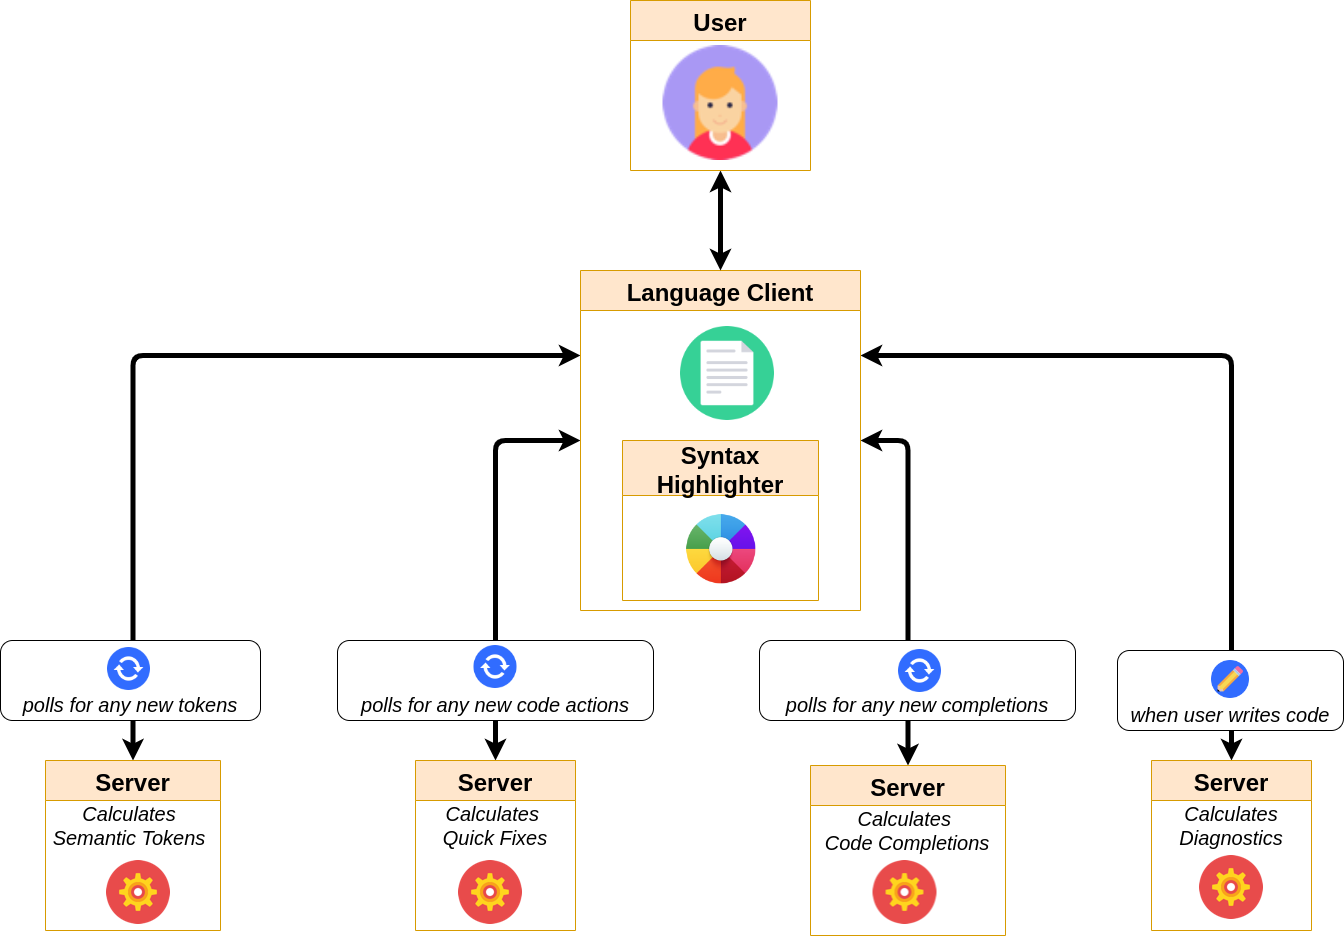
\includegraphics[width = \linewidth]{./figures/le-editor.png}
\caption{A diagram showing the overall structure of the Logical English editor.}
\label{fig:logo}
\end{figure}
The overall structure of the editor is as follows. The user interacts with the editor through the language client. The language client takes on the rules of the syntax highlighter to highlight basic syntactic features of the user's document. The language client highlights semantic features of the document, along with presenting any code completions or quick fixes, by routinely polling the language server for this data. The language server presents diagnostics by requesting diagnostic data from the server whenever the user makes a change to the document.

\section{Data Representation}
\subsection{Description of Problem}
When providing diagnostics, semantic highlighting, code completion or quick fixes, the initial task of the language server is always to extract the document's literals and templates. It was clear early on that this is the fundamental problem: the better the representation the editor has for the literals and templates, the easier all subsequent work on them will be. It was important to design representations that:
\begin{itemize}
    \item were lightweight: literals and templates would be reloaded every time the document received an update
    \item focused on semantics: it should be easy to perform queries and operations based on a literal's or template's meaning
    \item did not stray too far from the Logical English syntax: converting to and from Logical English should be simple
    \item were not too distinct from each other: templates and literals are often used together, such as querying whether a literal matches a template
\end{itemize}
Based on the last requirement, I could focus on first designing a representation for templates, and then use those ideas to design a similar representation for literals. 

\subsubsection{Initial Template Design}
Initially, the most obvious and simple design for a template was as a list of tokens, called `elements' \footnote{This is done to distinguish these tokens from the tokens used in highlighting the document}, each element being a string. These elements would either be a type, such as \codeword{*a person*}, or text that lies between the types, such as \codeword{goes shopping}. This list of elements was easily acheived by splitting a Logical English template by a regular expression that identified substrings of the form \codeword{*a _*} or \codeword{*an _*}. 
\\
\\
Although the design was lightweight and easy to implement, the more I used this design the clearer it became that it did not do enough work for me. Lots of duplicate work had to be re-done whenever this representation was used: specifically, identifying which elements are types, and filtering the list of elements to obtain each type, or each part of surrounding text. 
\\ 
\\
It became clear that, effectively, the list consisted of two different types of items: types, on the one hand, and surrounding text on the other. Based on this, the awkwardness of use, and the fact that I had plans to give types a richer structure, it was clear that the design needed upgrading, and it was also clear how.

\subsection{Element Representation}
The next level of abstraction was to abstract these two different kinds of elements into two different types.
The class \codeword{Type} was created to represent the type of a template argument. The class \codeword{Surrounding} was created to represent surrounding text that lies between types. As per my design philosophy, these are both lightweight types that store immutable values.

\subsection{Template Representation}
A template's elements were now a list of \codeword{TemplateElement} objects, where a \codeword{TemplateElement} is either a \codeword{Type} or a \codeword{Surrounding}.
The next logical step was to have a \codeword{Template} class to be a wrapper class around a \codeword{TemplateElement} list. This \codeword{Template} class provided a read-only view to the element list. It also exposed functions that queried the elements. These functions included obtaining the template's types or surrounding text -- what was previously done manually -- along with more advanced queries that will be discussed later.

\subsection{Literal Representation}
Once I had solved the \codeword{Template} design problem, I applied the same principles to creating a design for the literals. While working on the editor, I found that literals did not need as elaborate a design as templates: in fact, they did not even need their own class. In broad terms, a template acts on literals -- mainly through extracting terms, or checking whether a given literal matches its form. So, while templates have rich functionality, literals are passive objects that are acted on. There is no need to encapsulate a literal's elements behind a class, as a literal would not need any methods.
\\
\\
A Logical English literal consists of text that is either a term, or is surrounding text. So, similar to templates, the natural representation is a list of \codeword{LiteralElement} elements, where a \codeword{LiteralElement} is either a \codeword{Surrounding} or a \codeword{Term}.

\subsubsection{Term}
In logical english, a term is a value with an associated type. The natural data structure to represent this is therefore:
\begin{lstlisting}
    class Term:
        name: string
        type: Type
\end{lstlisting}
with each of these properties being immutable. It is important that the \codeword{type} property is a reference to the corresponding type, not a copy. This is crucial to see if two uses of the same Logical English term have conflicting types.

\subsection{Section Representation}
Along with representing Logical English data, it was also important to be able to refer to where the data lies in the document. This is crucial in highlighting features of the document, providing diagnostic error underlines and identifying the current literal that the user is typing. 
\\
\\
The immediate approach would have been to add a \codeword{range} field to each of the above classes, that specifies where the data begins and ends in the document. However, attaching range data to these representations themselves was a bad idea for two reasons: by the design principle of concerns \todo[inline]{Name the design principle} the representations are ``abstract'' in that they represent what a logical english construct is, not where it happens to lie in a document. Further, it is important to know where bodies of raw text (i.e. \codeword{string} objects) are. These do not have range data.

\subsubsection{ContentRange$<$T$>$}
The alternative solution was to have a class that wraps data, adding an additional range field. For a given type \codeword{T} (a \codeword{string}, a \codeword{Template} or any other kind of content), a \codeword{ContentRange<T>} has a \codeword{content} field of type \codeword{T}, and an immutable \codeword{range} field. 
\begin{lstlisting}
    class ContentRange<T>:
        content: T
        range: Range
\end{lstlisting}
The \codeword{range} field stores the beginning and the end of the content, in the \codeword{(line number, character number)} form that \codeword{vscode-langaugeserver} uses. 
\\
\\
Note that \codeword{T} could be any type whatsoever, including types that do not make sense (such as the \codeword{void} type, or the type of a function). However, there was not enough commonality between valid values of \codeword{T}, such as \codeword{string}, \codeword{Template} or \codeword{LiteralElement[]}, to constrain \codeword{T} effectively.
%
%
%
\section{Semantic Highlighting}
\subsection{An Overview}
The semantic highlighting highlights the terms of each atomic formula in the document. To identify the terms, the templates are first read from the document and represented as \codeword{Template} objects. For each literal, the \codeword{Template} object that best matches it is found by comparing each template against the literal. Using the closest-matching \codeword{Template} object, the literal's terms are identified and highlighted.

\subsection{How a Language Server highlights}
\todo[inline]{Research this in more detail}

% \subsection{Template Parsing}
% In parsing the templates, the lines containing templates are found, starting at the header \codeword{the templates are:}, and continuing until either another header or the end of the document is reached. 
% \\ 
% \\
% The \codeword{Template} class then constructs a template from each line. Each substring of the form \codeword{*a _*} or \codeword{*an _*} is taken to be a type name, and the corresponding \codeword{Type} object is put in the corresponding place. All other substrings are wrapped in a \codeword{Surrounding} object.

\subsection{Extracting the terms of a literal}
In short, the way I measure how well a template matches a literal is by assuming that the template does indeed match the literal, extracting the literal's elements according to this assumption, and judging the result. So I must first describe how a template extracts a literal's elements.
\\ 
\\
This is a fundamental problem that is used by many of the language server's features, such as type checking a literal's terms and ranking literal completions, along with semantic highlighting. This lead me to spend a long time trying different approaches to this problem.
\todo[inline]{Talk about these other algorithms and their limitations.}

The final algorithm leverages the assumption that the template and the literal share the same surroundings. Under this assumption, comparing the template's surroundings against the literal yields the literal's terms. The algorithm for this is given below.
\todo[inline]{Write up algorithm here}
This algorithm was constructed using the idea of incremental problem solving in my Algorithms course.
\todo[inline]{Expand on this.}
There is a slight subtlety here: what happens if a surrounding also appears as a term. For example, a scenario where a merchant packages and sends items could be described with the template \codeword{*a merchant* ships *an item*}. If we have a merchant who packages and sends ships, then the corresponding literal would be \codeword{the merchant ships ships}.
\todo[inline]{Describe how this nuance is handled}
\todo[inline]{Talk about how this algorithm works with the edge case of incomplete literals also}

\subsection{Matching a template to a literal}
Once all the template objects have been created, the templates can be used to highlight the terms in each literal. Starting with a given literal, the templates are filtered by whether or not they match the literal. 
\\
\\
Determining whether a template matches a literal is now a simple application of the algorithm that extracts the literal's elements. Once the literal's elements have been extracted, it suffices to check whether the literal's surroundings and the template's surroundings match.

\subsection{Finding the template that best matches a literal}
Initially, it was assumed that only one template can match a literal. This was convenient, as I could simply use the first (assumed only) template that matches the literal to identify the literal's terms. 
\\
\\
However, as the editor was being developed, I soon saw how this was often false. This was most clearly visible when ``default'' templates were implemented -- general templates, such as \codeword{*a thing* is *a thing*} that were implicitly present in every Logical English document. Consider the following Logical English document:
\begin{lstlisting}[langage={LE}]
the templates are:
*a thing* is *a thing*.
*a person* is a beneficiary of *a will*.

the knowledge base Counter-Example includes:
jane is a beneficiary of her father's will.
\end{lstlisting}
The first template to match the literal \codeword{jane is a beneficiary of her father's will} is the first template: \codeword{*a thing* is *a thing*}. However, this is not the template that \textit{should} match. In fact, using this template to extract the literal's terms will lead to 
\\ 
\\
This motivated a `match score' between a literal and a template. The higher the score, the better the template matches the literal, and the more certain we can be that it should be used to extract the terms.
\todo[inline]{Write up scoring algorithm}
\todo[inline]{Con: this is not normalised -- how are comparisons then meaningful?}
%
%
%
\section{Completion}
\subsection{How a language server completes code}
\todo[inline]{Research this in more detail}

\subsection{Completing the remainder of a literal}
To offer completion for a literal, first its corresponding templates are found. This is not as straightforward as searching for which templates match the literal, because the literal will be incomplete, and so will not match any template. Instead, the templates are ranked by their match score against the literal, and the top three are taken.
\\
\\
There is already some nuance here. Some matches will be ``obviously'' irrelevant, such as (the dreaded) \codeword{*a thing* is *a thing*} against \codeword{the person is a beneficiary of }. These cannot be ruled out algorithmically, however, since they do match. They will, however, be out-ranked by templates with better-matching surroundings, and will appear lower in the list.
Finding best three templates according to match score. Filling in templates with terms that the literal has so far.
\todo[inline]{Justify why at most three literals are suggested. Research user design.}
%
%
%
\section{Error diagnosis}
\subsection{How a language server diagnoses errors}
\todo[inline]{Research this in more detail}

\subsection{Diagnosing literals that have no matching template}
Given the above discussion it is fairly straightforward to find literals that do not match any template. The nuance is in using this as the deciding factor actually being too eager. Specifically, incomplete literals (e.g. literals that are being typed) will, in general, not match a template. This means that every literal that is being typed will be diagnosed as incorrect until it is finished.
\todo[inline]{Talk about how this is impossible to fix: on diagnosis time, all that is given is the text document, not the cursor position.}

\subsection{Diagnosing clauses that have misaligned connectives}
This is another problem that sounds simple in theory, once the above framework was developed, but turned out to have nuances in practice. Each clause is split into its lines, and the lines containing the keywords \codeword{and} and \codeword{or}, which have equal precedence, have their indentation compared. If two literals with different connectives have the same whitespace, then the precedence of the connectives is ambiguous.
\\
\\
The nuance is with the term `same indentation'. There are two equally common ways to indent lines: tabs and spaces. There is no standard way to display a tab in terms of spaces: any range from two to eight spaces is common. Thus, if one person indents literals using tabs, and the other using spaces, then it is up to interpretation as to whether the indent is correct or not.
\todo[inline]{Cite sources on this. Talk about how this is a problem in Python, and that there is no solution. Talk about how it should therefore be an error to mix spaces and tabs, but I do not want to check for this.}
Issue: spaces versus tabs

\subsection{Diagnosing type mismatches}

\subsubsection{Feature Overview}
Although not part of the editor's requirements, the Logical English development team wanted a way to introduce experimental support for typed terms. The argument labels in templates would give the type of their argument. This feature would be used for finding type errors in multiple uses of the same term across a clause. Since this feature is experimental, it was not supposed to clash with any existing features or hinder the experience of a user who did not want this.
\\
\\
The way I chose to implement this feature was to have type checking turned off by default, only being turned on with an explicit \codeword{type checking: on} comment. The type hierarchy was also designed to be as minimal as possible. 
\todo[inline]{Move this discussion to Requirements section.}

\subsubsection{Initial design: flat type hierarchy}
When experimenting with implementing this feature, I first implemented type checking before implemnting a type hierarchy. In each clause, the literals were extracted, and, using the document's templates, the terms were extracted from each literal. These terms were typed, but there was no notion of sub-type or super-type. If two terms were found that had the same name but different types, a type mismatch error message was generated.
\\ 
\\
This design was a lot more inconvenient to use than I expected, with many more surprising error messages being generated. This was mainly because of the default templates, and for two reasons. Firsly, since the default templates are very broad, they use placeholder type names, such as \codeword{A}, \codeword{B}, \codeword{C}, \codeword{thing}, et cetera. Ths caused problems for two reasons. Firstly, the type names clashed with the more specific type names found in real-world Logical English examples, if they were used together. Secondly, the type names often clashed amoungst themselves: take, for example, the template \codeword{*an A* appended to *a B* gives *a C*}, and the literal \codeword{[] appended to the list gives the list}. Here \codeword{the list} is both of type \codeword{B} and \codeword{C}.
\todo[inline]{Cite the default templates, or at least, talk about them in the LE specification.}
The solution to the first problem could only be resolved through a type hierarchy, making sure that the types used in the default templates would be super-types of whatever is used in more specific templates. However, the solution to the second problem was immediately resolvable: rename the types. All general type names such as \codeword{A}, \codeword{B}, \codeword{C} et cetera were renamed to \codeword{thing}.

\subsubsection{Diagnosing with a type hierarchy}
First, the type tree is read from the document under the header \codeword{the type hierarchy is:}. Parsing a text version of a tree is a well-known algorithmic problem.
\todo[inline]{Cite the solution.}
Now instead of simply checking whether two type names are equal, the two types are checked to see if one is a subtype of the other. Since types are rerpesented in a tree, this is a simple tree search problem to see whether either type node has a child node with the same name as the other type.
\todo[inline]{Cite the solution.}
%
%
%
\section{Quick Fixes}
\subsection{How a language server provides quick fixes}
\todo[inline]{Research this in more detail}

\subsection{Fixing a lack of template for literals}
\subsubsection{Template Generation using Least General Geneneralisation}
The first candidate template is generated according to the principle of least general generalisation. This is a principle from Logic-Based Learning which states how to generate a predicate that matches a set of given instantiations of the predicate, that is no more general than is necessary to match all of them.
\todo[inline]{Research and describe this more.}
The way this is done in the editor is as follows. Each literal is split into a list of space-separated words. It is assumed that there is a common template which matches all the literals. In the initial design, the predicate words were identified as the intersection of all the words. This criteria is slightly refined, and will be discussed later.
\\ 
\\
Having found all of the predicate words, the terms of the first literal are identified as the words that are not predicate words. Knowing both the predicate words and the terms of the first literal, I then generate a template that matches this. If this same template matches all the other literals, then it is returned.
\todo[inline]{Write up the algorithm.}

\subsubsection{Template Refinement from the re-use of terms}
It was often the case that the least general generalisation was not enough to generate an accurate template. Either there were too few example literals, or the examples did not vary every term. In trying to fix this problem, I noticed that I was not exploiting the context(i.e. the clause) in which the literal was written. If a literal borrows a term from another literal, then we know about that term, and can generalise it into a variable.
\\
\\
This was done by giving the \codeword{Template} class a method to generate a more general template by generalising a given term into a variable. Applying this method successively to all the surrounding terms that feature in each template-less literal gave much more accurate templates. This also allowed a single literal to be generalised into a template -- a feature that is impossible with least general generalisation. This also told us the type to place inside the template, since the type of each term is known.

\end{document}